\documentclass[conf]{new-aiaa}
%\documentclass[journal]{new-aiaa} for journal papers
\usepackage[utf8]{inputenc}

\usepackage{graphicx}
\usepackage{amsmath}
\usepackage{longtable,tabularx}
\usepackage{lettrine}
\setlength\LTleft{0pt}

\title{Graph Neural Networks for the Agile Earth Observation Satellite Scheduling Problem}

\author{Aiden Kampwerth\footnote{Student Researcher, Aerospace Engineering Department, Texas A\&M University}}

\begin{document}

\maketitle

\begin{abstract}
This report investigates the proposed use of Graph Decision Neural Networks (GDNN) with Proximal Policy Optimization (PPO) for the Agile Earth Observation Satellite Scheduling Problem (AEOSSP).
AEOSSP is a classical NP-hard problem with no exact solutions and therefore suboptimal solutions limit the usage and efficiency of Earth Observation Satellites (EOS) for a variety of image capturing tasks.
GDNN-PPO’s performance was investigated against traditional methods to solve AEOSSP by comparing Average Scheduling Profit, Average Scheduling Time, and Percentage of Excessive Profit across a range of task scales.
The analysis shows that GDNN-PPO improves solution quality by roughly 50\% relative to simple heuristics, achieves performance within about 7\% of state-of-the-art metaheuristic methods, and reduces solve time by more than two orders of magnitude while maintaining near-linear scaling in the number of tasks.
At the same time, the study identifies several modeling limitations, such as training on fixed problem sizes, simplified time-attitude graph construction, and incomplete use of critic information, that may restrict generalization and operational robustness.
The report concludes that graph-based RL provides a viable and computationally efficient framework for AEOSSP, and recommends concrete architectural and training modifications to further improve scalability and reliability for future agile Earth observation missions.
\end{abstract}

\section{Nomenclature}

{\renewcommand\arraystretch{1.0}
\noindent\begin{longtable*}{@{}l @{\quad=\quad} l@{}}
$N$  & number of observation tasks \\
$t$  & time \\
AEOS   & Agile Earth Observation Satellite \\
AEOSSP & Agile Earth Observation Satellite Scheduling Problem \\
CDTD   & Conflict Degree of Task Descending \\
CNN    & Convolutional Neural Network \\
DQN    & Deep Quality Network \\
EOS    & Earth Observation Satellite \\
GDNN   & Graph Decision Neural Network \\
GNN    & Graph Neural Network \\
GRILS  & Greedy Randomized Iterated Local Search \\
LEO    & Low Earth Orbit \\
PPO    & Proximal Policy Optimization \\
PTD    & Profit of Task Descending \\
RL     & Reinforcement Learning \\
RPID   & Ratio of Profit and Image time Descending \\
SDE    & Self-adaptation Differential Evolution \\
SGA    & Self-adaptation Genetic Algorithm \\
SOTA   & State of the Art \\
STWA   & Start time of observational Time Window Ascending \\
VTW    & View Time Window \\
\end{longtable*}}

\section{Introduction}

\subsection{Agile Earth Observation Satellites}
In recent years, a combination of lowering launch costs and increased payload sizes to Low Earth Orbit (LEO) has enabled the use of larger and more numerous satellite systems for a wide variety of scientific endeavors.
Consequently, a new generation of Earth Observation Satellites (EOS) have been developed and deployed to meet the growing demand of observation tasks from the scientific community which range from wildfire detection\cite{shams2025assessing}, sea surface temperature tracking\cite{minnett2019half}, and glacier movements\cite{raup2015remote}.
More specifically, the development of Agile Earth Observation Satellites (AEOS), which now provide three degrees of freedom for tracking, enable the study of numerous, unrelated tasks across the entire observable view of the satellite.

\subsection{Non-Polynomial Hard Optimization}
Choosing an optimal ordering to perform each task within time and energy constraints is a combinatorial difficult NP-Hard problem, akin to the classical Traveling Salesman problem\cite{lawler1991traveling}.
While exact solutions to the Agile Earth Observation Satellite Scheduling Problem (AEOSSP) exist, they remain computationally intractable for even a moderately large number of tasks.
Approximately optimal greedy heuristics exists however they often fail to reach sufficient parody with the exact solution while remaining computationally expensive.
This has therefore necessitated the development of new state-of-the-art optimizers capable of solving AEOSSP within computational and time-constrained bounds onboard spacecraft.

\begin{figure}[hbt!]
\centering
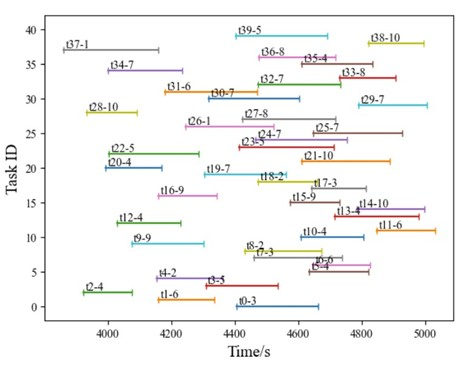
\includegraphics[width=.8\textwidth]{task_id_vs_time}
\caption{Normally distributed sample of possible observation tasks \cite{chun2023deep}.}
\label{fig:task_distribution}
\end{figure}

\subsection{Reinforcement Learning}
A key innovation is Reinforcement Learning (RL), a new paradigm championed by Google DeepMind's AlphaGo\cite{silver2016mastering}, which achieved superhuman level play in the Chinese game of Go.
Fundamentally, RL mimics the rewards-based mechanisms within the human brain to learn general solutions to complex tasks through self-taught evolution.
Learning is typically split between two components of a single agent, the actor network and the critic network.
The actor takes actions within a state space that ideally maximizes an arbitrary value function controlled by the critic.
The critic then learns from the actor’s actions to update the value function to more accurately represent the state space’s rewards.
In laymen’s terms, the critic computes the possible decisions and their consequences, and the actor decides how to choose between the possible decisions for the best reward.
Over many iterations, an RL agent near optimally generates its own training set by balancing exploration and exploitation as well as assigning rewards to the training set based on its own perceived value, solving the additional constraints placed on a graph-based optimal solver.

\begin{figure}[hbt!]
\centering
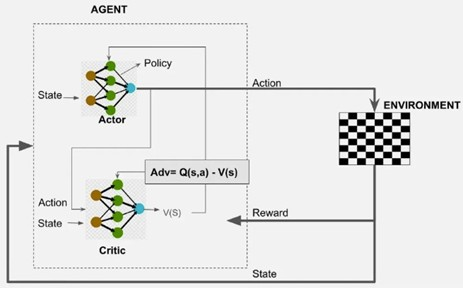
\includegraphics[width=.8\textwidth]{reinforcement_learning_diagram}
\caption{Simplified RL agent with reward system \cite{chun2023deep}.}
\label{fig:rl_agent}
\end{figure}

\section{Objective}
To construct a more optimal solver, AEOSSP can be reframed as a causally directed graph network with a time dimension and three spatial (rotation angle) dimensions\cite{lemaitre2002selecting,peng2020solving}.
A graph network is a set of nodes (features of interest) connected via edges (relationships between features) which represent some arbitrarily abstract collection of information.
In AEOSSP, nodes represent observation tasks and edges represent time (and consequently energy) constraints between each task\cite{scarselli2009graph,bronstein2017geometric}.
For AEOSSP, it is valuable to understand how future rewards (completing tasks) can be achieved through choosing certain paths earlier as the most optimal total rewards may not be guaranteed if the maximal next reward is the only criteria (greedy algorithms).
Therefore, it is natural to formulate AEOSSP as a graph problem for which numerous machine learning models can approximate an optimal solver.

\begin{figure}[hbt!]
\centering
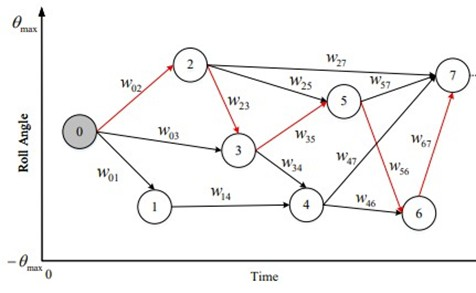
\includegraphics[width=.8\textwidth]{graph_network_roll_angle_vs_time}
\caption{Simplified graph of AEOSSP with 1 degree of freedom \cite{chun2023deep}.}
\label{fig:aeossp_graph}
\end{figure}

Subsequently, the primary success criteria are to:
\begin{enumerate}
\item Scale efficiently to task sizes beyond approximately 27 tasks limit of exact solvers
\item Achieve accuracy surpassing traditional approximate solvers and heuristics
\item Respect time and energy constraints of observable windows and available onboard propellant
\item Generalize well beyond training set examples
\item Remain computationally tractable for on-orbit satellites to compute
\end{enumerate}

\section{GDNN-PPO Framework}

\subsection{Graph Decision Neural Networks}
To address these constraints, a Graph Decision Neural Network (GDNN) RL agent architecture was proposed by Chun, et al.\cite{chun2023deep}.
GDNNs are a minor modification to the classical Graph Neural Network (GNN) found throughout the machine learning field.
A GNN’s basic principle is to share node information across connected edges to fully contextualize all the information in a graph, similar to how Convolutional Neural Networks (CNN) work but on an irregular grid.
Information is spread in “message passing” rounds where nodes aggregate information provided by their neighbors to add as a residual on the current stored information.
Information can therefore propagate through a graph over several rounds of message passing to result in a final contextualized state of the graph.
In AEOSSP, this framework allows future tasks to inform prior tasks about their characteristics which theoretically enables the current task to understand the context several tasks in the future given only the next available tasks.
Given the contextualized model, the GNN is modified to contain a final output layer to decide between the potential next available tasks (a GDNN) which is then used to update the graph to the next state.
GNN models are inherently based on supervised learning which assumes a training set with accurate rewards (or labels) that are absent from the current formulation of the solver.
Therefore, RL was proposed to generate the necessary training set (and associated test set) to construct the solver.

\begin{figure}[hbt!]
\centering
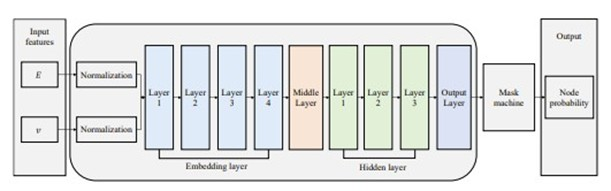
\includegraphics[width=.8\textwidth]{graph_decision_neural_network_model_architecture}
\caption{Graph Decision Neural Network model architecture \cite{chun2023deep}.}
\label{fig:gdnn_architecture}
\end{figure}

\subsection{Proximal Policy Optimization Framework}
The RL agent framework utilizes GDNN as primary model around which it optimizes.
A single GDNN provides the primary structure (backbone) for both the actor and critic networks with separate final output layers for the actor and critic.
Proximal Policy Optimization (PPO)\cite{schulman2017proximal} objective was utilized to train both networks in tandem.
Standard Policy Optimization (PO) maximizes the expected reward of a series of actions over a set horizon (number of tasks) with a weighting parameter favoring maximizing current rewards vs future rewards.
PPO improves upon standard Policy Optimization by computing the ratio of current achieved rewards to previously achieved rewards, clipping this ratio to prevent large model weight updates, significantly stabilizing training.

As a high-level overview, the actor GDNN encodes the list of tasks into a graph representation which is passed through the model to decide on the next task.
The satellite then moves to perform that task (under the time and energy constraints encoded in the nodal information) which represents the updated graph state.
This then repeats until the satellite reaches the final target time when the total rewards are accumulated based on the value assigned from the critic GDNN.
The rewards are then used to update the actor and then critic weights to reflect the information learned through the training set and the cycle is repeated until the framework reaches the convergence criteria.
The Average Scheduling Profit (ASP), the Average Scheduling Time (AST), and Percentage of Excessive Profit (PSP) are compared against other methods to determine the most optimal method.

\begin{figure}[hbt!]
\centering
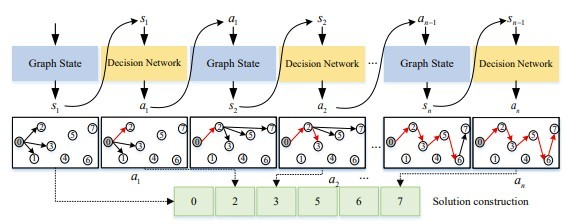
\includegraphics[width=.8\textwidth]{actor_gdnn_constructing_solution_graph}
\caption{Actor GDNN constructing a solution subgraph \cite{chun2023deep}.}
\label{fig:actor_subgraph}
\end{figure}

\section{Performance Evaluation}

\subsection{Baseline Heuristics}

The four standard heuristics were utilized as a baseline benchmark:
\begin{enumerate}
\item Start time of observational Time Window Ascending (STWA) --- tasks ordered by start time
\item Profit of Task Descending (PTD) --- prioritizes most rewarding tasks
\item Ratio of Profit and Image time Descending (RPID) --- measures reward per time spent on task
\item Conflict Degree of Task Descending (CDTD) --- targets most clustered tasks first
\end{enumerate}

As expected, the heuristics perform poorly against the machine learning based models as they necessarily ignore important aspects of AEOSSP as seen in Figure 6.
Despite the poor performance, the heuristics provide valuable information about AEOSSP.
Specifically, the heuristics perform similarly (within tens of relative percent of each other) while optimizing for significantly different criteria.
Therefore, it can be concluded that task availability, reward value, task duration, and spatial and temporal separation all remain important to AEOSSP and, consequently, all valid solvers must respect each of these aspects.

\begin{figure}[hbt!]
\centering
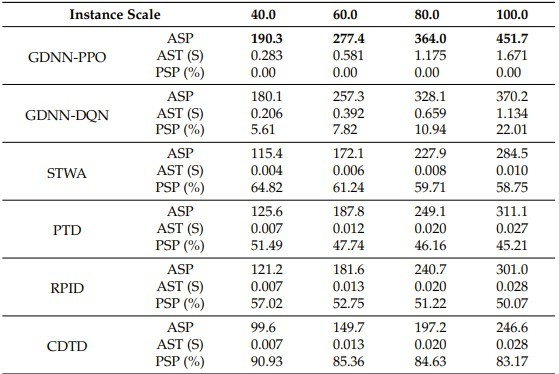
\includegraphics[width=.8\textwidth]{model_accuracy_comparison}
\caption{Comparison of GDNN-PPO against simple models \cite{chun2023deep}.}
\label{fig:comparison_simple}
\end{figure}

\subsection{State-of-the-Art Comparison}
More accurate methods such as GRILS, Self-adaption Differential Evolution (SDE), and Self-adaptation Genetic Algorithm (SGA) were compared against in Figure 7.
Notably, GDNN-PPO (referred to as GAT-PPO in Figure 7) falls behind the most optimal model, GRILS, in the ASP metric which would violate the objective of the GDNN-PPO model except that GRILS scales poorly with task scale as seen in Figure 8 with AST scores rapidly increasing with task scale.
Filtering for only scalable models, GDNN-PPO significantly out-performs its only competition, SGA, and therefore satisfies the constraints set above.
Based off these results, it was concluded that the GDNN-PPO proposed satisfies the original objective criteria and suggests that efforts to improve scheduling priority should be investigated.

\begin{figure}[hbt!]
\centering
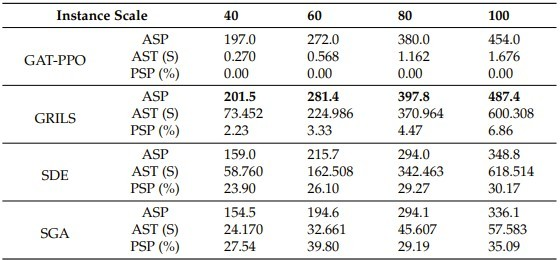
\includegraphics[width=.8\textwidth]{model_comparison_sota}
\caption{Comparison of GDNN-PPO against SOTA models \cite{chun2023deep}.}
\label{fig:comparison_sota}
\end{figure}

\begin{figure}[hbt!]
\centering
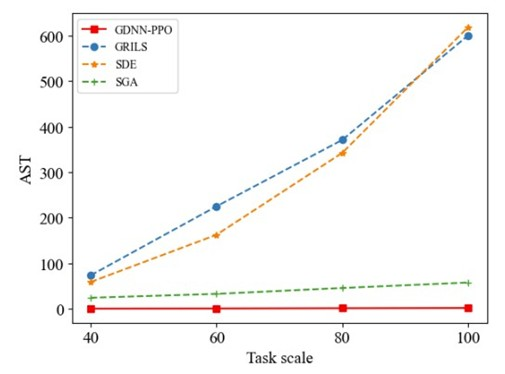
\includegraphics[width=.8\textwidth]{ast_vs_task_scale}
\caption{Solve time against task scale \cite{chun2023deep}.}
\label{fig:solve_time}
\end{figure}

\section{Proposed Implementation}

\subsection{Training set construction}
The construction of the training set is done at a single task scale at a time with which the model is trained on.
This necessarily restricts the model to learning how to optimize over a set horizon rather than learning a generalized solution over an indefinite horizon, a distinction which the literature acknowledges through comparison of the GDNN-PPO model trained and tested at varying scales.
Given the model’s ability to train and test on differing task scales, a natural improvement to the model would be the inclusion of a variety of task scales in the model’s environment.
It follows that a scale-invariant GDNN-PPO would necessarily improve the generalizability to a wide variety of task scales as expected in realworld deployment.
Combining a variety of task scales could also be done gradually throughout the training procedure with the introduction of larger task scales only after the model has begun understanding smaller cases.
This method could additionally promote stability in training which random shuffling of task sizes may erode.

\subsection{Graph modeling}
The graph modeling of AEOSSP is done via a time-attitude adjacency graph where distances are computed via a time heuristic equation that only incorporates the roll angle while ignoring pitch and yaw angles.
Furthermore, the edge connections are generated via a five-nearest neighbors computation performed in the time heuristic domain.
While theoretically sufficient, the graph modeling approach is both simple and restrictive to the information naturally stored within each task.
Incorporating all three angles via the transition angle equation already defined likely improves the model’s understanding of the true mechanics without sacrificing any time constraints which are validated later in the process.
Furthermore, adding additional nodal information related to the constraints, such as slack time to the View Time Window (VTW) end when transitioning nodes, may aid the model’s ability to select subgraphs which prevent dead ends.

\subsection{RL framework}
The RL framework lacks a proper description of the critic network, a crucial aspect of the RL architecture, and thus is assumed to be an identical model structure to the actor network (GDNN).
The actor and critic model are assumed to have independent encoding structures (embedding layers) which typically hurt alignment between the actor and critic, harming generalization.
Utilizing a shared encoding structure between actor and critic with separate GNN layer blocks both unifies the learned representation of the agent as well as maintains the representability of the individual networks.
Furthermore, adding regularization to the critic, such as L2 loss or physics-informed losses, may provide increased stability or accuracy over training while maintaining or improving the generalizability of the model.
Additionally, removing infeasible transitions between tasks creates sharp gradients during training which are not immediately visible compared to when infeasible transitions are utilized directly in the reward structure.
Adding constraint-based losses with smooth gradients (PPO-Lagrangian) may improve training and generalizability to optimal strategies rather than pattern exploitation.

\section{Conclusion}
The Agile Earth Observation Satellite Scheduling Problem presents a difficult challenge that the rapidly growing space industry needs to tackle to fully utilize the increasing demand from a variety of customers.
Traditionally methods and heuristics fall short in either solution quality or generation speed which limit the operational effectiveness of satellites.
A GDNN-PPO approach proposed achieved the objective in producing high-quality solutions to AEOSSP while remaining computationally tractable yet still left open numerous avenues for improvement of the algorithm as well as expansion to more challenging versions of AEOSSP.

GDNN-PPO achieved approximately 50\% increase in model performance compared to basic heuristics and fell within 7\% of SOTA heuristics-based methods while maintaining near linear scaling on task size and remaining within 2 second solve time.
The 350x reduction in solve time compared to SOTA methods represents fundamental shift from pure research to practical implementation.
Furthermore, the success of the model proposed suggests similar classes of NP-Hard problems can approximately solved in real-time, a potentially revolutionary possibility.

Despite the tantalizing benefits, indirect limitations of GDNN-PPO hamper the overall benefit of the model.
Modeling decisions such as task scale-locked environments, neglected beneficial node and edge information, and lack of proper RL framework implementation suggest major improvements are still available.

Even with current model, practical implementation remains feasible.
Adoption into practical applications might involve a range of deployments from scheduled settings with human oversight to fully autonomous systems onboard satellites able to handle requests from a variety of users.
Faster, more efficient, more productive Earth observation satellites have moved from a mathematically impossible problem to an engineering implementation possibility.

\bibliography{individual_assignment}

\end{document}
